\documentclass[a0paper,portrait]{baposter}

\usepackage{wrapfig}
\usepackage{lmodern}
\usepackage[french]{babel}
\usepackage{lipsum,graphicx}
\usepackage[utf8]{inputenc} %unicode support
\usepackage[T1]{fontenc}\usepackage{geometry}
\usepackage{geometry}
\usepackage{ragged2e}
\usepackage{setspace}
\usepackage[font=footnotesize,labelfont=bf,skip=0pt,justification=centering]{caption}
\captionsetup[figure]{labelfont={bf},labelformat={default},labelsep=period,name={Fig.}}
\selectcolormodel{cmyk}

\graphicspath{{figures/}} % Directory in which figures are stored

\newcommand{\compresslist}{%
\setlength{\itemsep}{0pt}%
\setlength{\parskip}{1pt}%
\setlength{\parsep}{0pt}%
}

\newenvironment{boenumerate}
  {\begin{enumerate}\renewcommand\labelenumi{\textbf\theenumi.}}
  {\end{enumerate}}
  \geometry{top=22pt, bottom=10pt}
  \hyphenation{sur-production résistance respiratoire apnées bronchiolite symptomatique relative désencombrer}


\begin{document}

\definecolor{Mycolor1}{HTML}{00FFFF}
\definecolor{Mycolor2}{HTML}{008080}

\begin{poster}
{
grid=false,
headerborder=open, % Adds a border around the header of content boxes
colspacing=0.8em, % Column spacing
bgColorOne=Mycolor2, % Background color for the gradient on the left side of the poster
bgColorTwo=Mycolor2, % Background color for the gradient on the right side of the poster
borderColor=Mycolor1, % Border color
headerColorOne=Mycolor2, % Background color for the header in the content boxes (left side)
headerColorTwo=Mycolor2, % Background color for the header in the content boxes (right side)
headerFontColor=white, % Text color for the header text in the content boxes
boxColorOne=white, % Background color of the content boxes
textborder=rounded, %rectangle, % Format of the border around content boxes, can be: none, bars, coils, triangles, rectangle, rounded, roundedsmall, roundedright or faded
eyecatcher=true, % Set to false for ignoring the left logo in the title and move the title left
headerheight=0.08\textheight, % Height of the header
headershape=rounded, % Specify the rounded corner in the content box headers, can be: rectangle, small-rounded, roundedright, roundedleft or rounded
headershade=plain,
headerfont=\Large\textsf, % Large, bold and sans serif font in the headers of content boxes
%textfont={\setlength{\parindent}{1.5em}}, % Uncomment for paragraph indentation
linewidth=2pt % Width of the border lines around content boxes
}
{}
%
%----------------------------------------------------------------------------------------
%	TITLE AND AUTHOR NAME
%----------------------------------------------------------------------------------------
%
{
\textsf %Sans Serif
{
{\textcolor{white}{Tout savoir sur la bronchiolite aiguë \\ du nourrisson}}
}
} % Poster title
% {\vspace{0.2em} Add Author Name, Add another author name\\ 
% {\small \vspace{0.7em} Department of Computing, TU Dublin, Tallaght, Dublin, Ireland}} 
{\sf\vspace{0.1em}\\
\textcolor{white}{{Julian Belotti, Guillaume Deside, Anaïs Volondat} \- \footnotesize{(Groupe 3)}}  % Author names
\vspace{0.1em}\\
\small{ \textcolor{white}{LGBIO 1113 Anatomie et physiologie des systèmes}
\vspace{0.1em} % Author email addresses
\\
}
}
{
\includegraphics[width=.3\linewidth]{images/UCLouvain_logo.png}}


% this states the box starts at column 0 (edge of page), row 0 (top of page) for a span of 3 (columns wide)
\headerbox{1.Introduction}{name=introduction,column=0,row=0, span=3}{
\vspace{0.2cm}
\begin{minipage}{\linewidth}
\begin{wrapfigure}[10]{r}{0.5\textwidth}
\vspace{-15pt}
\includegraphics[width=\linewidth]{images/épidémie.png}
\caption{Nombre d'hospitalisations en France}
\end{wrapfigure}
\vspace{0.3}
\RaggedRight
La bronchiolite aiguë est une \textbf{\mbox{maladie inflammatoire}} touchant les \textbf{bronchioles}. Elle est d’origine \textbf{\mbox{virale}}, \mbox{généralement} causée par le virus \mbox{respiratoire} syncytial. \\Cette maladie est très \textbf{contagieuse} mais bénigne dans la majorité des cas. Environ \textbf{30\%} des nourrissons tombent \textbf{malade} chaque année et seulement
\textbf{2\%} de ceux-là sont \textbf{hospitalisés}.\\
La \textbf{transmission} se fait par les \textbf{sécrétions} de la personne malade.\\
La maladie sévit sous forme d'\textbf{épidémie} d'octobre à avril dans l'hémisphère Nord.
\end{minipage}
\vspace{0.1cm}
}

% this states the box starts at column 0 (edge of page), directly below the box labelled introduction for a span of 1 (column wide)
\headerbox{2.Anatomie et physiopathologie}{name=subtopic1,column=3,row=0,span=2}{
\vspace{0.2cm}
\begin{minipage}{\textwidth}
\begin{wrapfigure}{R}{0.35\textwidth}
\vspace{-15pt}
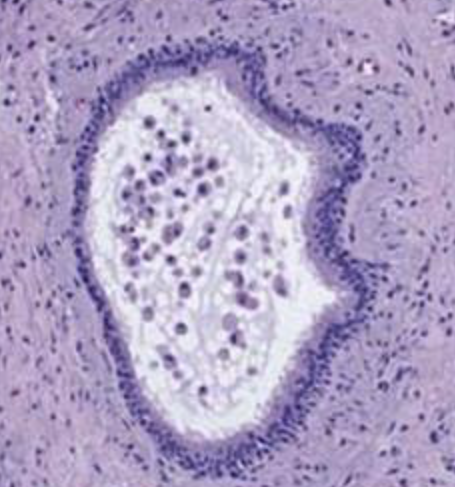
\includegraphics[width=\linewidth]{images/normale.png}
\vspace{-10pt}
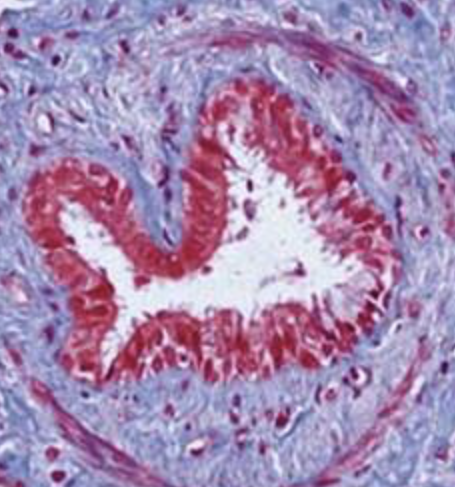
\includegraphics[width=\linewidth]{images/malade.png}
\vspace{0.2}
\caption{Bronchiole saine et malade}
\end{wrapfigure}
\RaggedRight
Les \textbf{bronchioles} appartiennent au \textbf{système respiratoire inférieur}. Elles sont entourées par du \textbf{muscle lisse} et ont un \textbf{épithélium cylindrique simple cilié}. Elles ne possèdent pas de cartilage. \\Leur rôle est d'assurer le \textbf{passage de gaz} jusqu’aux \textbf{alvéoles}.\\
La bronchiolite est l'\textbf{obstruction} des bronchioles provoquée par le \textbf{plissement} et un \textbf{oedème} des \textbf{muqueuses}, une \textbf{surproduction} de \textbf{mucus}, et des \textbf{bronchospasmes}. La \textbf{réduction} de la \textbf{lumière augmente} la \textbf{résistance} du système respiratoire et donc le travail nécéssaire à la ventilation des alvéoles.
\end{minipage}
\vspace{0.1cm}
}

% symptomes

\headerbox{3.Symptômes et traitements}{name=subtopic3,column=0,below=introduction,span=3}{
  \begin{minipage}{\linewidth}

    \begin{wrapfigure}{l}{0.43\textwidth}
        \includegraphics[width=\linewidth]{images/viscosité.png}
      \includegraphics[width=\linewidth]{images/équation.png}
      \includegraphics[width=\linewidth]{images/unités.png}
      \vspace{-0.3cm}
      \caption{Relation entre viscosité et résistance à l'écoulement de l'air}
      \vspace{-1pt}
    \end{wrapfigure}

    \textbf{\textcolor{Mycolor1}{}}\\
    {\large{\textbf{\textcolor{Mycolor1}{Symptômes}}}}
    \RaggedRight
    \vspace{0.1cm}
    
La bronchiolite se manifeste en premier lieu par une \textbf{toux sèche}, un \textbf{rhume} et parfois de la \textbf{fièvre}. \\
Puis, les symptômes évoluent : la \textbf{toux} s'intensifie et \textbf{devient grasse}, les sécrétions qui s’accumulent dans les bronchioles provoquent davantage de \textbf{difficultés respiratoires}. Celles-ci se manifestent par une \textbf{polypnée}, un \textbf{tirage intercostal}, un \textbf{wheezing}.\\
Les symptômes \textbf{disparaissent}, \textbf{généralement}, \textbf{naturellement} au bout de quelques jours.
Cependant, il est \textbf{possible} que l’état du nourrisson ne s’améliore pas et qu’une \textbf{hospitalisation} soit \textbf{nécessaire}. Les signes sont : des \textbf{apnées}, un \textbf{refus de s’alimenter}, une \textbf{cyanose}, des \textbf{étourdissements} ou \textbf{évanouissements}. Ces symptômes sont dus à une \textbf{hypoxémie}.
\end{minipage}
\\
\\
\\
\begin{minipage}{\linewidth}
    \begin{wrapfigure}{r}{0.6\textwidth}

        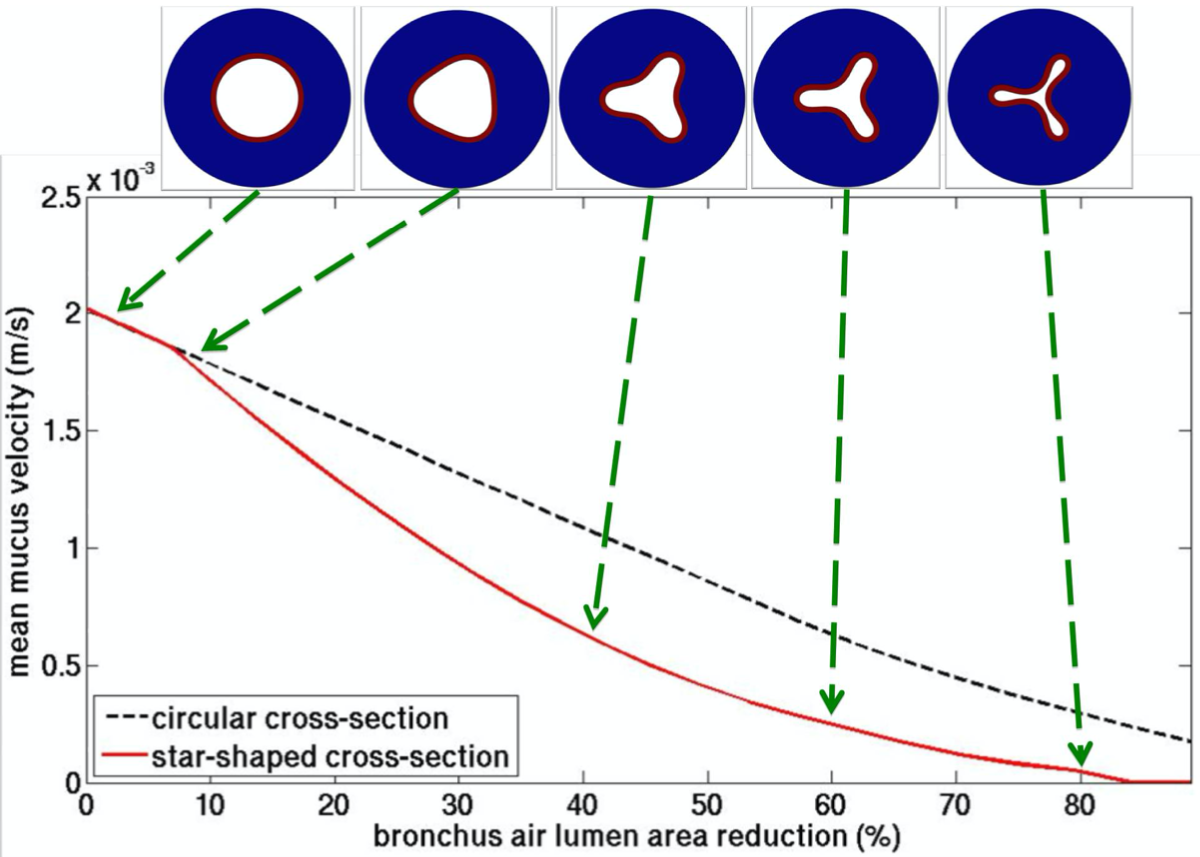
\includegraphics[width=\linewidth]{images/vitesse.png}
        \caption{Vitesse du mucus en fonction de l'aire de la lumière}
        \vspace{-1cm}
    \end{wrapfigure}
\vspace{0.6cm}


    \textbf{\textcolor{Mycolor1}{}}\\
    {\large{\textbf{\textcolor{Mycolor1}{Traitements}}}}
    \RaggedRight
    \vspace{0.1cm}

Les traitements de la bronchiolite sont purement \textbf{symptomatiques}.\\
\vspace{0.1cm}
\textbf{\textcolor{Mycolor2}{Bronchiolite aiguë sans \mbox{hospitalisation}}}\\
\vspace{0.03cm}
Afin de \textbf{soulager} l’enfant, de nombreux gestes sont conseillés :\\
- \textbf{Hydrater} abondamment \\ \ \  l’enfant.\\
- \textbf{Fractionner} les \textbf{repas} et \\ \ \ \textbf{épaissir} le lait du \textbf{biberon}.\\
- \textbf{Moucher} le nourrisson.\\
- Bien \textbf{aérer la chambre} et \\ \ \ \mbox{réduire} sa température à \textbf{19°c}.\\
- Avoir recours à la \textbf{kinésithérapie respiratoire}.\\
\vspace{0.1cm}
\textbf{\textcolor{Mycolor2}{Bronchiolite aiguë avec hospitalisation}}\\
\vspace{0.03cm}
Des traitements supplémentaires sont nécessaires :\\
- L’\textbf{apport d’oxygène} si la saturation en oxygène du nourrisson est inférieure à 94\%.\\
- Les \textbf{antibiotiques} en cas de forte fièvre ou de surinfection.\\
- Les \textbf{bronchodilatateurs}. Les spécialistes ne s’accordent pas tous sur ce traitement.

\end{minipage}
\vspace{0.1cm}
}
%Kiné
\headerbox{4.Kinésithérapie respiratoire}{name=kine,column=3,span=2,below=subtopic1}{
\vspace{0.2cm}
\begin{minipage}{\linewidth}

    \begin{wrapfigure}{r}{0.63\textwidth}
      \vspace{-15pt}
      \begin{center}
        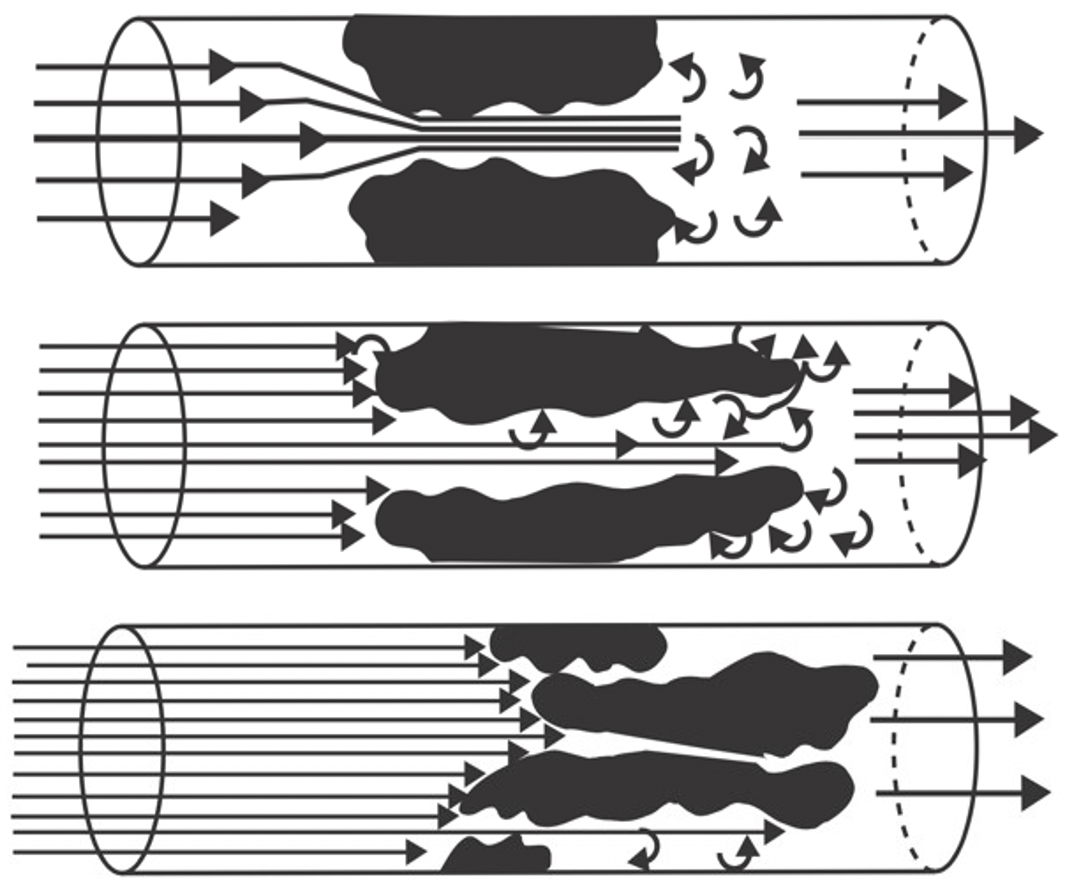
\includegraphics[width=\linewidth]{images/AFE.png}
        \caption{Augmentation du flux expiratoire}
      \end{center}
              \vspace{-20pt}
    \end{wrapfigure}
    \RaggedRight
    L'\textbf{objectif} principal des séances de kinésithérapie respiratoire (KR) est de \textbf{désencombrer} les bronchioles/bronches.\\
Les spécialistes ne la prescrivent pas tous car elle \textbf{améliore} l’état du nourrisson à \textbf{court terme} mais \textbf{ne réduit pas} la \textbf{période de guérison}.\\
Les techniques pratiquées sont l’\textbf{expiration passive}, \textbf{lente} ; la \textbf{toux provoquée} ; l’\textbf{augmentation du flux expiratoire}.
\vspace{0.15cm}
\end{minipage}
\RaggedRight
\textbf{\textcolor{Mycolor1}{Rôle de l'ingénieur}}\\
\vspace{0.03cm}
La \textbf{KR} est très \textbf{\mbox{controversée}}. L'ingénieur pourrait \textbf{modéliser} les \textbf{flux} dans les poumons lors de séances de KR. Cela permettrait d'observer les effets de celle-ci et de \textbf{juger} de son \textbf{\mbox{efficacité}}. 
C'est l'objectif du projet \mbox{« VirtualChest} – poumon numérique pour la kinésithérapie respiratoire ».
\vspace{0.1cm}
}
%tomo

\headerbox{5.Tomodensitométrie}{name=topicoverview,column=3,span=2,below=kine}{
\vspace{0.2cm}
\begin{minipage}{\linewidth}

    \begin{wrapfigure}{l}{0.49\textwidth}
      \vspace{-16pt}
      \begin{center}
        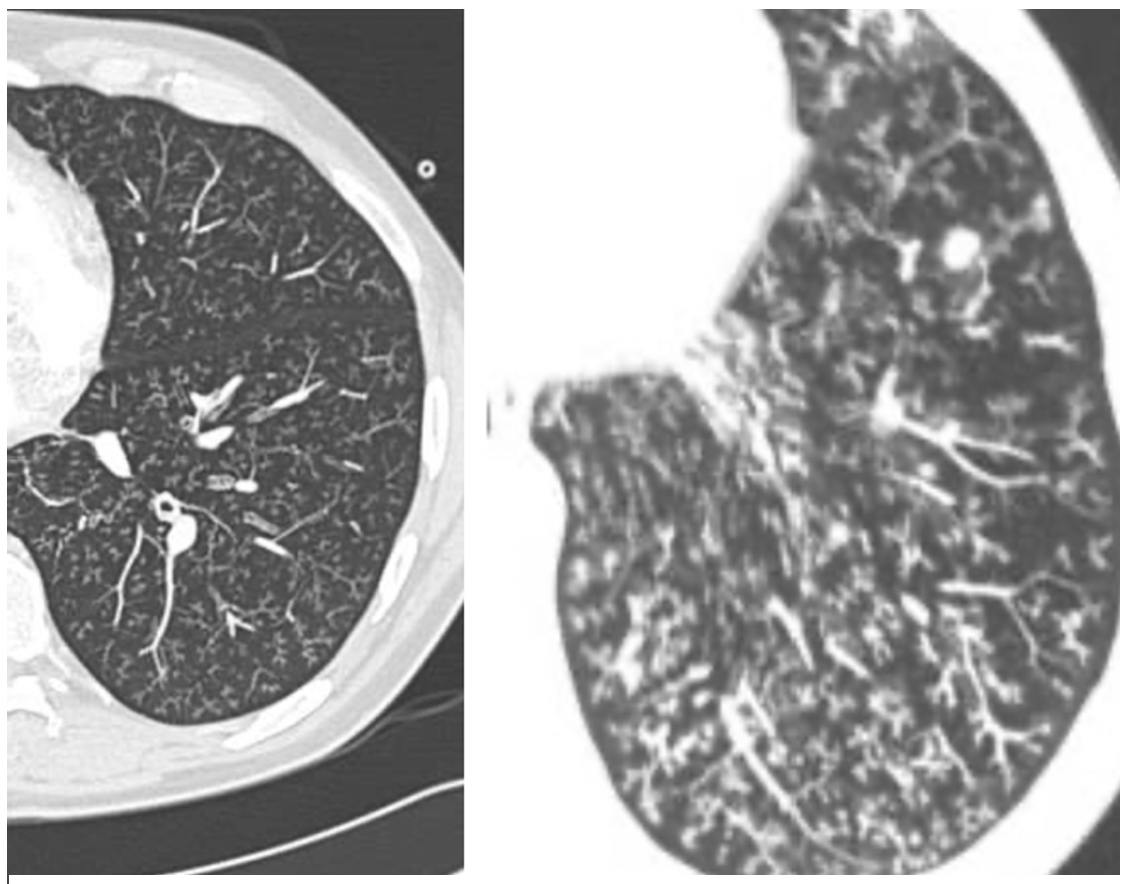
\includegraphics[width=\linewidth]{images/micronodules.png}
        \includegraphics[width=\linewidth]{images/mosaïque.png}
        \caption{Images de TDM}
      \end{center}
      \vspace{-1cm}
    \end{wrapfigure}
\RaggedRight
La tomodensitométrie (TDM) est une technique d’imagerie médicale.
La TDM \textbf{détecte} les \textbf{bronchioles} (visibles sous forme de \mbox{micronodules}), invisibles chez les personnes \mbox{saines ;} l'\textbf{épaisseur} anormale de la \textbf{paroi} bronchique (visible sous forme d’arbre bourgeonnant) ; la \textbf{répartition inégale de l’air} dans les poumons (visible sous forme de zones hypodenses et en mosaïque).\\
\vspace{0.05cm}
\textbf{\textcolor{Mycolor1}{Rôle de l'ingénieur}}\\
\vspace{0.03cm}
Si les bronchioles sont \textbf{trop sévèrement atteintes}, la TDM \textbf{ne détecte pas} le \textbf{piégeage de l'air}. L'ingénieur pourrait trouver un moyen afin de le détecter même si celui-ci est très prononcé.
\end{minipage}
\vspace{0.1cm}
}


\headerbox{6.Conclusion}{name=conclusion,column=0,below=subtopic3,span=3, bottomaligned=topicoverview}{

\RaggedRight
Même si la bronchiolite est une \textbf{maladie très fréquente} chez le nourrisson, \mbox{celle-ci} reste \textbf{peu étudiée} et \textbf{mal connue}. L’absence de consensus international en est la preuve.
Les seuls traitements qui existent sont symptomatiques et les \textbf{médecins ne s’accordent pas} sur les techniques et les solutions de \textbf{traitement}.\\
Du fait de la relative méconnaissance de cette pathologie, l’\textbf{ingénieur} a un \textbf{réel rôle} à jouer dans la \textbf{recherche} de \textbf{solutions} et la \textbf{compréhension} de la bronchiolite.\\
\vspace{0.05cm}
{\footnotesize \textbf{Reférences}}\\
\vspace{0.1cm}
\begin{spacing}{0.01}
{\tiny Friedmann, J. N., Rieder, M. J., & Walton, J. M. (2014). La bronchiolite : Recommandations pour le diagnostic, la surveillance et la prise en charge des enfants de un à 24 mois.}
\end{spacing}\\
\vspace{0.05cm}
\begin{spacing}{0.01}
{\tiny Jeckel, S. (2012, octobre). Nouvelles recommandations sur la prise en charge de la bronchiolite du nourrisson : état des lieux dans un service de pédiatrie à l’hôpital Notre Dame de Bonsecours à METZ (57000), saison hiver 2011/2012.}
\end{spacing}
}

\end{poster}

\end{document}

 